
\documentclass[11pt]{article}
\usepackage{style/acl2016}
\usepackage{titlesec}
\usepackage{graphicx}
\usepackage{amsmath}
\usepackage{subfig}
\usepackage{times}
\usepackage{url}
\usepackage{latexsym}
\usepackage{breakurl}

\makeatletter
\newcommand{\@BIBLABEL}{\@emptybiblabel}
\newcommand{\@emptybiblabel}[1]{}
\makeatother

\usepackage[bookmarks=false,
pdfpagelabels=false,
hyperfootnotes=false,
hyperindex=false,
pageanchor=false,
]{hyperref}

\makeatletter
\let\saved@hyper@linkurl\hyper@linkurl

\let\saved@hyper@link@\hyper@link@
\AtBeginDocument{
  
  
  \NoHyper
  
  
  
}



\aclfinalcopy 






\newif\ifcomment\commentfalse
% Preamble file contains handy macros and most packages you might want to use.
% At the start are packages that conflict with various styles.  Don't add them
% in!  Just put it in your main TeX file instead.

% Do not put either of these (subfigure or subfloat) into the preamble
% - they clash.  Use them in the final LaTeX document
% \usepackage{subfigure}
% \suepackage{subfloat}

% Do not use times in the preamble!  It just causes problems with some
% publication chairs (e.g., ICML 2013).  If you want it, put it in your own
% document.
% \usepackage{times}


% Breaks ACM-SIG style
% \usepackage{titlesec}
% \usepackage{amsthm}
% \usepackage{nomencl}

% comment out the following line, as it conflicts with aistats2012.sty
%\usepackage{caption}


% Below should be safe
\usepackage{framed}
\usepackage{mdwlist}
\usepackage{latexsym}
\usepackage{xcolor}
\usepackage{nicefrac}
\usepackage{booktabs}
\usepackage{amsfonts}
\usepackage{bold-extra}
\usepackage{amsmath}
\usepackage{dsfont}
\usepackage{amssymb}
\usepackage{bm}
\usepackage{graphicx}
\usepackage{mathtools}
\usepackage{microtype}
\usepackage{multirow}
\usepackage{multicol}
%\usepackage{url}
\usepackage{latexsym,comment}

\newcommand{\breakalign}{\right. \nonumber \\ & \left. \hspace{2cm}}



\newcommand{\feat}[1]{{\small \texttt{#1}}}
\newcommand{\act}[1]{{\small \texttt{#1}}}
\newcommand{\ngram}[0]{$n$-gram}
\newcommand{\topic}[1]{\underline{#1}}
\newcommand{\gem}[1]{\mbox{\textsc{gem}}}
\newcommand{\abr}[1]{\textsc{#1}}
\newcommand{\camelabr}[2]{{\small #1}{\textsc{#2}}}
\newcommand{\abrcamel}[2]{{\textsc #1}{\small{#2}}}
\newcommand{\grammar}[1]{{\color{red} #1}}
\newcommand{\explain}[2]{\underbrace{#2}_{\mbox{\footnotesize{#1}}}}
\newcommand{\dir}[1]{\mbox{Dir}(#1)}
\newcommand{\bet}[1]{\mbox{Beta}(#1)}
\newcommand{\py}[1]{\mbox{\textsc{py}}(#1)}
\newcommand{\td}[2]{\mbox{\textsc{TreeDist}}_{#1} \left( #2 \right)}
\newcommand{\yield}[1]{\mbox{\textsc{Yield}} \left( #1 \right)}
\newcommand{\mult}[1]{\mbox{Mult}( #1)}
\newcommand{\wn}{\textsc{WordNet}}
\newcommand{\twentynews}{\textsc{20news}}
\newcommand{\g}{\, | \,}
\newcommand{\Gam}[1]{\Gamma \left( \textstyle #1 \right)}
\newcommand{\LG}[1]{\log \Gamma \left( \textstyle #1 \right)}
\newcommand{\Pois}[1]{\mbox{Poisson}(#1)}
\newcommand{\pcfg}[3]{#1_{#2 \rightarrow #3}}
\newcommand{\grule}[2]{#1 \rightarrow #2}
\newcommand{\kl}[2]{D_{\mbox{\textsc{KL}}} \left( #1 \,||\, #2 \right)}

\newcommand{\digambig}[1]{\Psi \left( #1 \right) }
\newcommand{\digam}[1]{\Psi \left( \textstyle #1 \right) }
\newcommand{\ddigam}[1]{\Psi' \left( \textstyle #1 \right) }

\DeclareMathOperator*{\argmax}{arg\,max}
\DeclareMathOperator*{\argmin}{arg\,min}
\newcommand{\bmat}[1]{\text{\textbf{#1}}}
\newcommand{\bvec}[1]{\boldsymbol{#1}}

\newcommand{\email}[1]{ {\small \href{mailto://#1}{\texttt{#1} }  }}
\newcommand{\emaillink}[2]{ {\small \href{mailto://#2}{\texttt{#1} }  }}

\newcommand{\ch}[1]{\begin{CJK*}{UTF8}{gbsn}#1\end{CJK*}}

\newcommand{\e}[2]{\mathbb{E}_{#1}\left[ #2 \right] }
\newcommand{\h}[2]{\mathbb{H}_{#1}\left[ #2 \right] }
\newcommand{\ind}[1]{\mathds{1}\left[ #1 \right] }
\newcommand{\ex}[1]{\mbox{exp}\left\{ #1\right\} }
\newcommand{\D}[2]{\frac{\partial #1}{\partial #2}}
\newcommand{\elbo}{\mathcal{L}}

\newcommand{\hidetext}[1]{}
\newcommand{\ignore}[1]{}

\newcommand{\todo}[1]{\textcolor{red}{{\bf TODO: #1}}}

\ifcomment
\newcommand{\pinaforecomment}[3]{\colorbox{#1}{\parbox{.8\linewidth}{#2: #3}}}
\else
\newcommand{\pinaforecomment}[3]{}
\fi

\newcommand{\jbgcomment}[1]{\pinaforecomment{red}{JBG}{#1}}
\newcommand{\mjpcomment}[1]{\pinaforecomment{blue}{MJP}{#1}}
\newcommand{\czcomment}[1]{\pinaforecomment{orange}{chen}{#1}}
\newcommand{\ffcomment}[1]{\pinaforecomment{red}{FF}{#1}}
\newcommand{\fpcomment}[1]{\pinaforecomment{green}{FP}{#1}}
\newcommand{\yhcomment}[1]{\pinaforecomment{green}{YH}{#1}}
\newcommand{\hhecomment}[1]{\pinaforecomment{blue}{HH}{#1}}
\newcommand{\tncomment}[1]{\pinaforecomment{blue}{TN}{#1}}
\newcommand{\mnicomment}[1]{\pinaforecomment{green}{Mohit}{#1}}
\newcommand{\prcomment}[1]{\pinaforecomment{lightblue}{Pedro}{#1}}
\newcommand{\fscomment}[1]{\pinaforecomment{orange}{Shi}{#1}}
\newcommand{\vmcomment}[1]{\pinaforecomment{yellow}{Varun}{#1}}
\newcommand{\rscomment}[1]{\pinaforecomment{yellow}{Richard}{#1}}
\newcommand{\jszcomment}[1]{\pinaforecomment{green}{JSG}{#1}}
\newcommand{\ascomment}[1]{\pinaforecomment{blue}{AS}{#1}}
\newcommand{\vecomment}[1]{\pinaforecomment{blue}{VE}{#1}}
\newcommand{\halcomment}[1]{\pinaforecomment{magenta!20}{Hal}{#1}}
\newcommand{\kgcomment}[1]{\pinaforecomment{blue}{Kim}{#1}}
\newcommand{\vancomment}[1]{\pinaforecomment{green}{VAN}{#1}}
\newcommand{\thangcomment}[1]{\pinaforecomment{green}{Thang}{#1}}
\newcommand{\alvincomment}[1]{\pinaforecomment{cyan}{Alvin}{#1}}
\newcommand{\reviewercomment}[1]{\pinaforecomment{blue}{Reviewer}{#1}}
\newcommand{\brscomment}[1]{\pinaforecomment{blue}{BRS}{#1}}
\newcommand{\psrcomment}[1]{\pinaforecomment{yellow}{PSR}{#1}}
\newcommand{\zkcomment}[1]{\pinaforecomment{cyan}{ZK}{#1}}
\newcommand{\swcomment}[1]{\pinaforecomment{yellow}{SW}{#1}}
\newcommand{\shaycomment}[1]{\pinaforecomment{yellow}{SBC}{#1}}
\newcommand{\jlundcomment}[1]{\pinaforecomment{cyan}{J}{#1}}
\newcommand{\kdscomment}[1]{\pinaforecomment{ceil}{KDS}{#1}}
\newcommand{\lkfcomment}[1]{\pinaforecomment{yellow}{LF}{#1}}
\newcommand{\yfcomment}[1]{\pinaforecomment{brown}{YF}{#1}}
\newcommand{\ewcomment}[1]{\pinaforecomment{lightblue}{Eric}{#1}}

\newcommand{\smalltt}[1]{ {\tt \small #1 }}
\newcommand{\smallurl}[1]{ \begin{tiny}\url{#1}\end{tiny}}
%\newcommand{\smallurl}[1]{ \begin{tiny} HIDDEN \end{tiny}}
\newenvironment{compactenum}{ \begin{enumerate*} \small }{ \end{enumerate*} }

\definecolor{lightblue}{HTML}{3cc7ea}
\definecolor{CUgold}{HTML}{CFB87C}
\definecolor{grey}{rgb}{0.95,0.95,0.95}
\definecolor{ceil}{rgb}{0.57, 0.63, 0.81}


% Datasets

\newcommand{\qb}[0]{Quizbowl}
\newcommand{\triviaqa}{\camelabr{Trivia}{qa}}
\newcommand{\qblink}{\abrcamel{qb}{Link}}
\newcommand{\qanta}{\textsc{qanta}}

\newcommand{\name}[0]{\abr{alto}}


\addtolength\titlebox{.5in}


 
\newcommand{\sect}[1]{\label{sec:#1} \input{sections/#1}}

\newcommand\BibTeX{B{\sc ib}\TeX}
\title{ALTO: Active Learning with Topic Overviews for Speeding Label Induction and Document Labeling}
\author{Forough Poursabzi-Sangdeh, \\
              {\bf Jordan Boyd-Graber} \\
              Computer Science \\
	     University of Colorado\\
	    \smalltt{forough.poursabzisangdeh@colorado.edu} \\
	    \smalltt{Jordan.Boyd.Graber@colorado.edu}
	\And
	 {\bf Leah Findlater}\\
         iSchool and \abr{umiacs} \\
	 University of Maryland\\
	\smalltt{leahkf@umd.edu}
	\And
	 {\bf Kevin Seppi} \\
         Computer Science \\
	 Brigham Young University\\
	\smalltt{kseppi@cs.byu.edu}
	}



\begin{document}

\maketitle

\begin{abstract}
  Effective text classification requires experts to annotate data with
  labels; these training data are time-consuming and expensive to
  obtain. If you know what labels you want, active learning can reduce
  the number of labeled documents needed.  However, establishing the label
  set remains difficult. Annotators often lack the global knowledge
  needed to induce a label set.  We introduce \name{}: Active Learning
  with Topic Overviews, an interactive system to help humans annotate
  documents: topic models provide a global overview of what labels to
  create and active learning directs them to the right documents to
  label.  Our user study with forty annotators shows that while active
  learning by itself is best in extremely resource limited conditions,
  topic models (even by themselves) lead to better label sets, and
  \name{}'s combination is best overall.
\end{abstract}

\section{Introduction}
\label{sec:introduction} Many fields depend on texts labeled by human experts; computational
linguistics uses such annotation to determine word senses and
sentiment~\cite{wordsense,sentiment}; while social science uses
``coding'' to scale up and systemetize content
analysis~\cite{policy_pref_Budge,policy_pref_Klingemann}.

Classification takes these labeled data as a training set and labels new data
automatically.  Creating a broadly applicable and consistent 
label set that generalizes well is time-consuming
and difficult, requiring expensive annotators to examine large swaths
of the data. Effective \abr{nlp} systems must
measure~\cite{hwa2004sample,osborne2004ensemble,ngai2000rule} and
reduce annotation cost~\cite{tomanek2007approach}. Annotation is hard because it requires both \emph{global}
and \emph{local} knowledge of the entire dataset.  Global knowledge is
required to create the set of labels, and local knowledge is required
to annotate the most useful examples to serve as a training set for an
automatic classifier.

We create a single interface---\name{} (Active Learning with Topic
Overviews)---to address both the global and local challenges using two machine
learning tools: \emph{topic models} and \emph{active learning} (we review both
in Section~\ref{sec:ALTO}). Topic models address the need for annotators to have
a \emph{global overview} of the data, exposing the broad themes of the corpus so
annotators know what labels to create.  Active learning \emph{selects} documents that
help the classifier understand the differences between labels and directs
the user's attention \emph{locally} to them.  We thus create four experimental
conditions to compare the effects of providing users with either a topic model
or a simple list of documents, with or without active learning suggestions
(Section~\ref{sec:conditions}). Following this section we then describe our data
and evaluation metrics (Section~\ref{sec:data_metrics}).
















Through both synthetic experiments (Section~\ref{sec:synthetic_exp}) and a user
study (Section~\ref{sec:user_exp_results}) with 40 participants, we evaluate
\name{} and its constituent components by comparing results from the four
conditions introduced above.  We first examine user strategies for organizing
documents, user satisfaction, and user efficiency. Finally, we evaluate the overall effectiveness of the label set in a post study crowdsourced task. 






\section{\name{}: Active Learning with Topic Overviews}
\label{sec:ALTO} 
\begin{table}[t!]
\small
\begin{tabular}{ p{2.4cm}  p{4.3cm} }
    \hline
    Topic words & Document Title
    \tabularnewline \hline \hline

metropolitan, carrier, rail, freight, passenger, driver, airport, traffic, transit, vehicles &
A bill to improve the safety of motorcoaches, and for other purposes.
    \tabularnewline
    \hline
	violence, sexual, criminal, assault, offense, victims, domestic, crime, abuse, trafficking
		& A bill to provide criminal penalties for stalking.
\tabularnewline
\hline
agricultural, farm, agriculture, rural, producer, dairy, crop, producers, commodity, nutrition
		& To amend the Federal Crop Insurance Act to extend certain supplemental agricultural disaster assistance programs through fiscal year 2017, and for other purposes.
\tabularnewline
\hline
\end{tabular}
\caption{
  Given a dataset---in this case, the \abr{us} congressional bills
  dataset---topics are automatically discovered sorted lists of terms that summarize segments of a document collection.  Topics also
  are  associated with documents.  These topics give users a
  sense of documents' main themes and help users create high-quality labels.}
\label{tab:doc_topics}
\end{table}


This section details \name{}:\footnote{
\let\hyper@linkurl\saved@hyper@linkurl
Code available at \url{https://github.com/Foroughp/ALTO-ACL-2016}
\NoHyper } a framework for assigning labels to
documents that uses both global and local knowledge to help users
create and assign document labels. We explain how
\name{} uses topic models to aid label induction and document
labeling. We then use active learning to direct user attention and
speed document labeling.











\paragraph{Topic Models}

Topic models~\cite{Blei-03} automatically induce structure from a text
corpus.  Given a corpus and a constant $K$ for the number of topics,
topic models output (i) a distribution over words for each topic $k$
($\phi_{k,w}$) and (ii) a distribution over topics for each document
($\theta_{d,k}$).  Each topic's most probable words and associated
documents can help a user understand what the collection is
about. Table~\ref{tab:doc_topics} shows examples of topics and their
highest associated documents from our corpus of \abr{us} congressional
bills.

Our hypothesis is that showing documents grouped by topics will be more effective
than having the user wade through an undifferentiated list of random documents and
\emph{mentally sort the major themes themselves}.













\paragraph{Active Learning}

Active learning~\cite{settles2012active} directs users' attention to
the examples that would be most useful to label when training a
classifier.  When user time is scarce, active learning builds a
more effective training set than random labeling: uncertainty
sampling~\cite{lewis1994sequential} or query by
committee~\cite{seung1992query} direct users to the most useful
documents to label.

In contrast to topic models, active learning provides local
information: this is the individual document you should pay attention
to.  Our hypothesis is that active learning, when used as a
\emph{preference function} to direct the users to documents most
beneficial to label, will not only be more effective than randomly
selecting documents but will also \emph{complement} the global
information provided by topic models. Section~\ref{sub:AL} describes
the preference functions for the experimental conditions.









\section{Study Conditions}
\label{sec:conditions} 
\begin{figure*}[t!]

  \begin{center}
  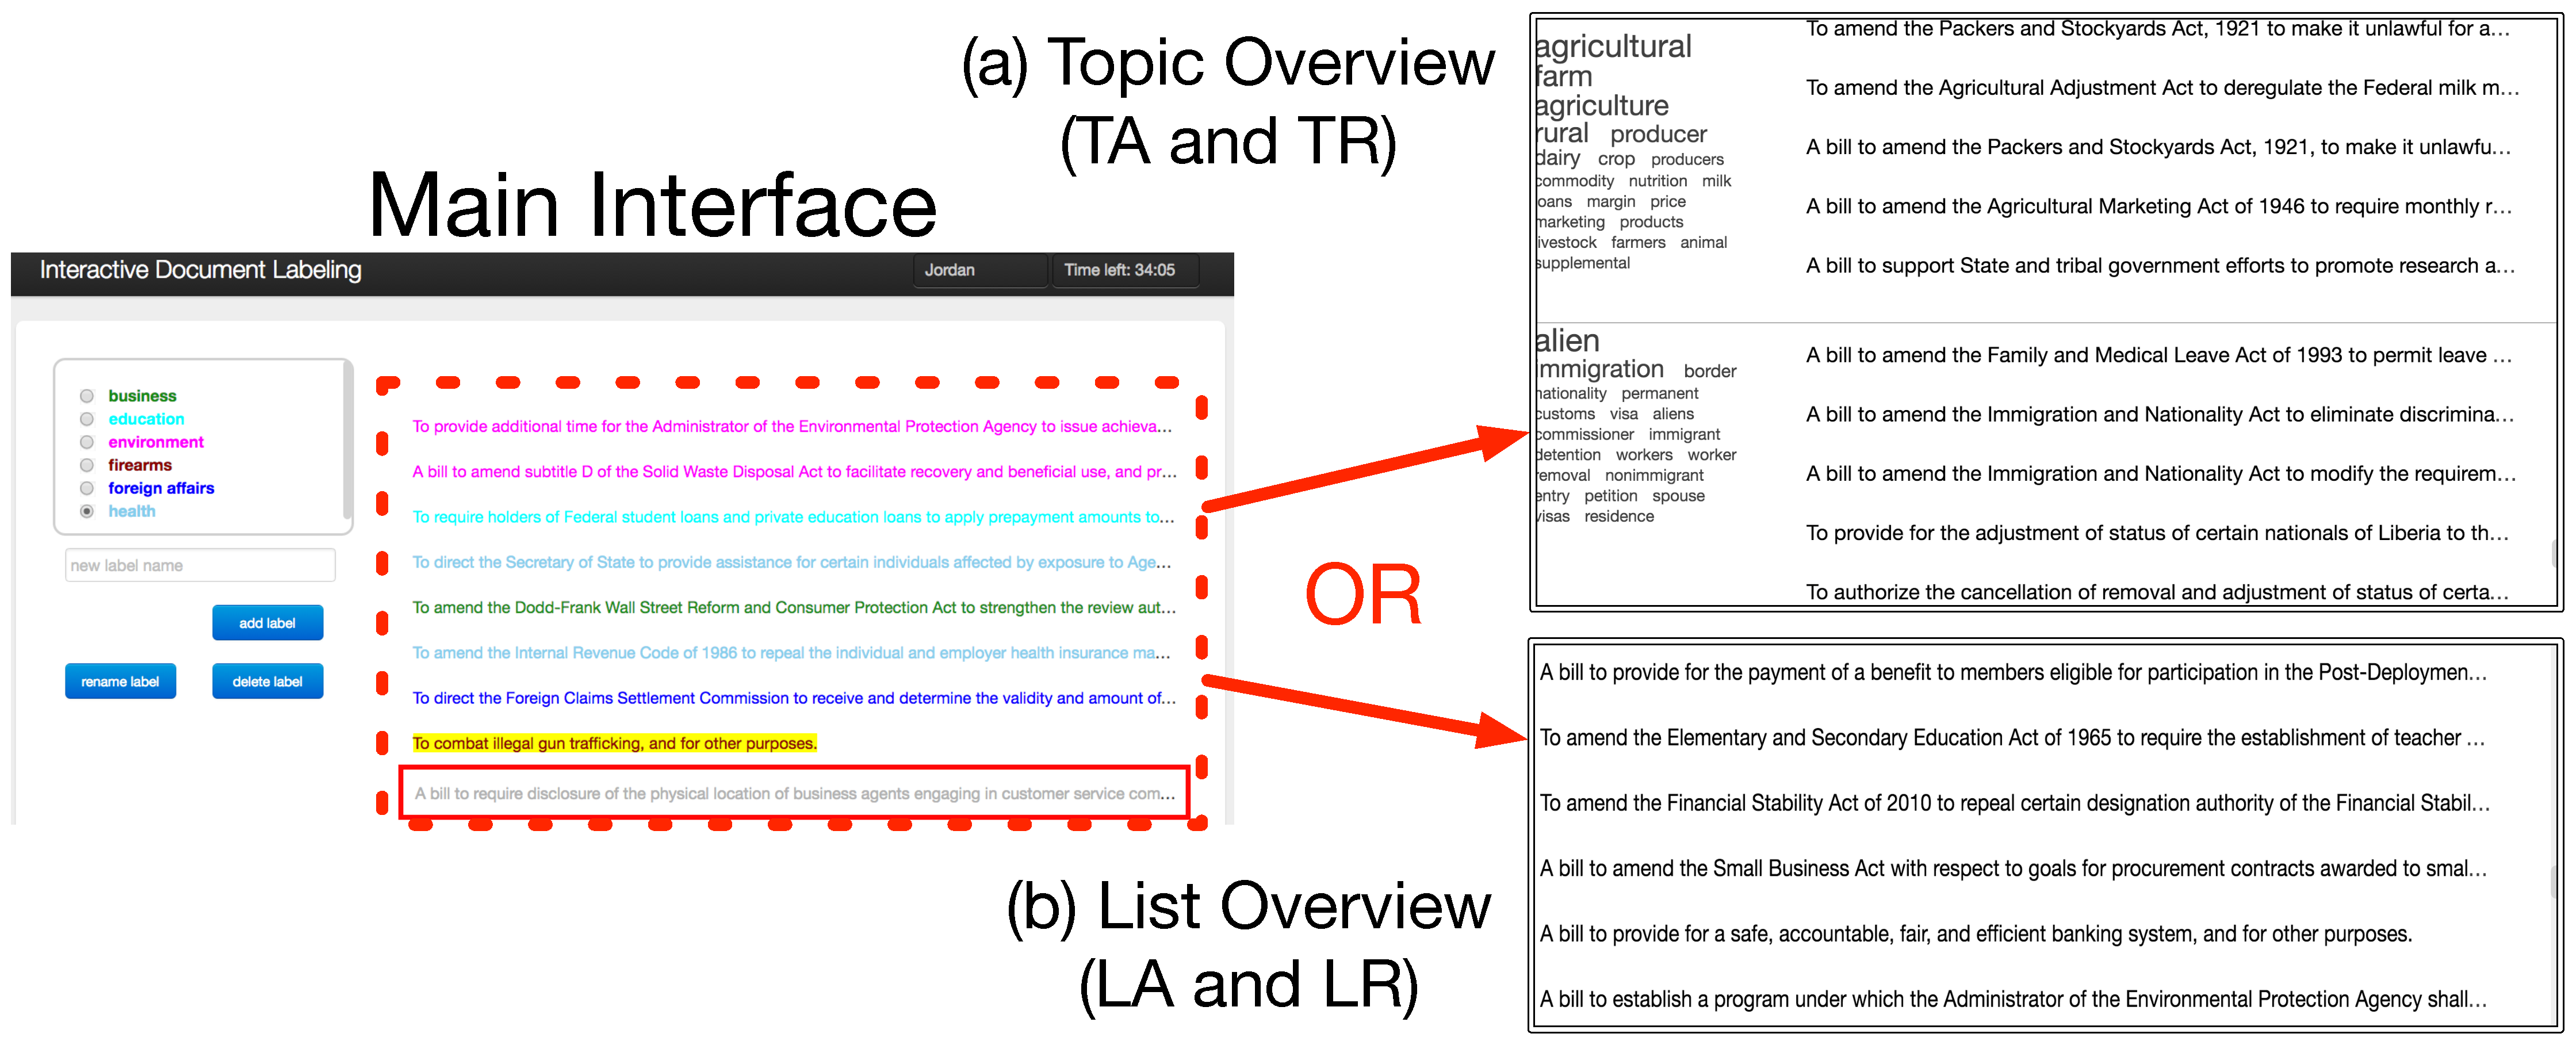
\includegraphics[width=\textwidth]{2016_acl_doclabel/figures/ui_docview}
  \end{center}

	\caption{Our annotation system.  Initially, the user sees lists of
          documents organized in either a list format or grouped into
          topics (only two topics are shown here; users can scroll to
          additional document).  The user can click on a document to
          label it.}
\label{fig:UI-overview}
\end{figure*}

\begin{figure}[t!]

  \begin{center}
  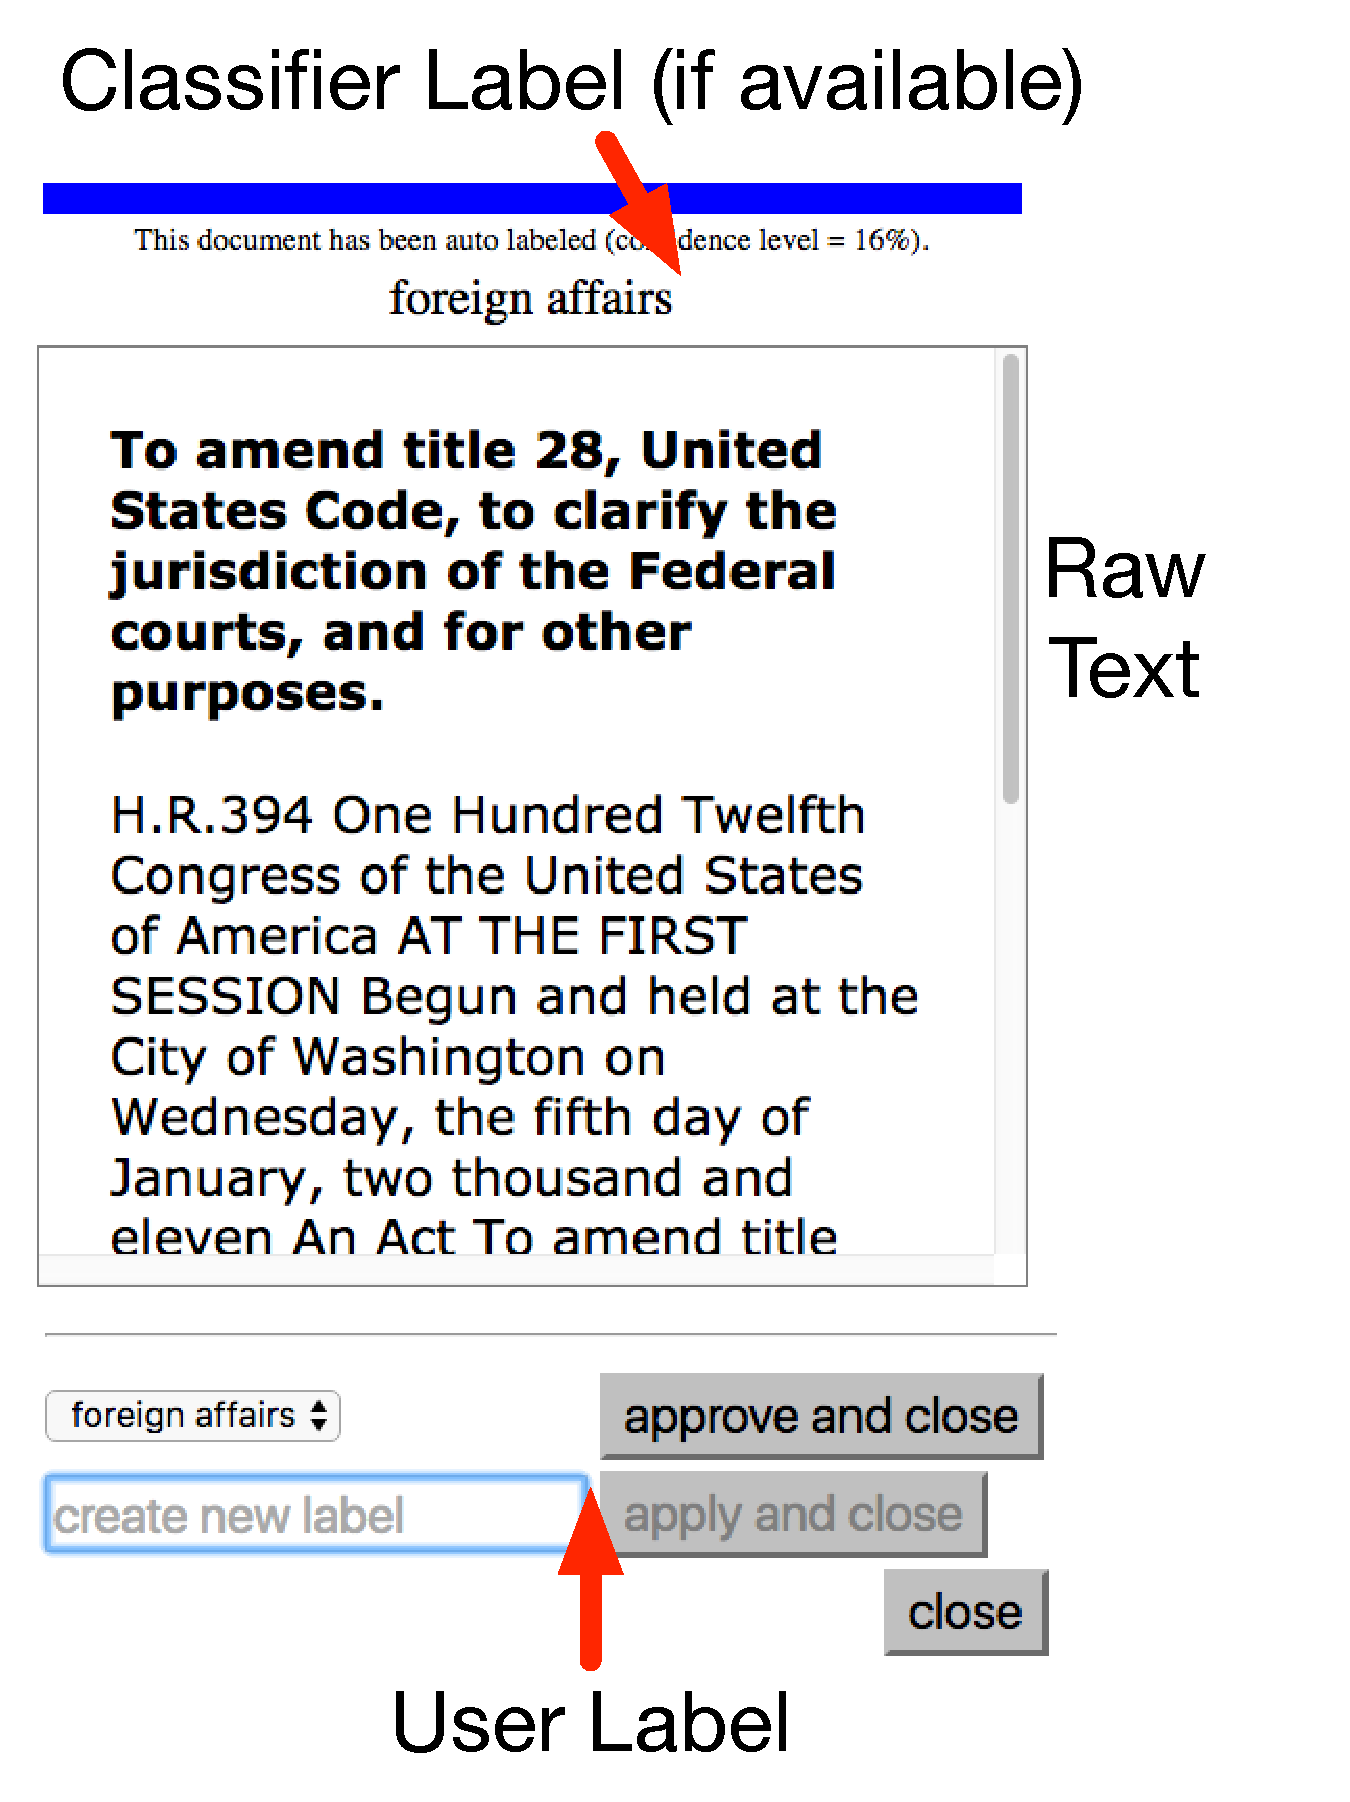
\includegraphics[width=.7\linewidth]{2016_acl_doclabel/figures/UI_labeling}
  \end{center}

	\caption{After clicking on a document from the list or
          topic overview, the user inspects the text and provides
          a label.  If the classifier has a guess at the
          label, the user can confirm the guess.}
\label{fig:UI-label}
\end{figure}

\begin{figure}[t!]

  \begin{center}
  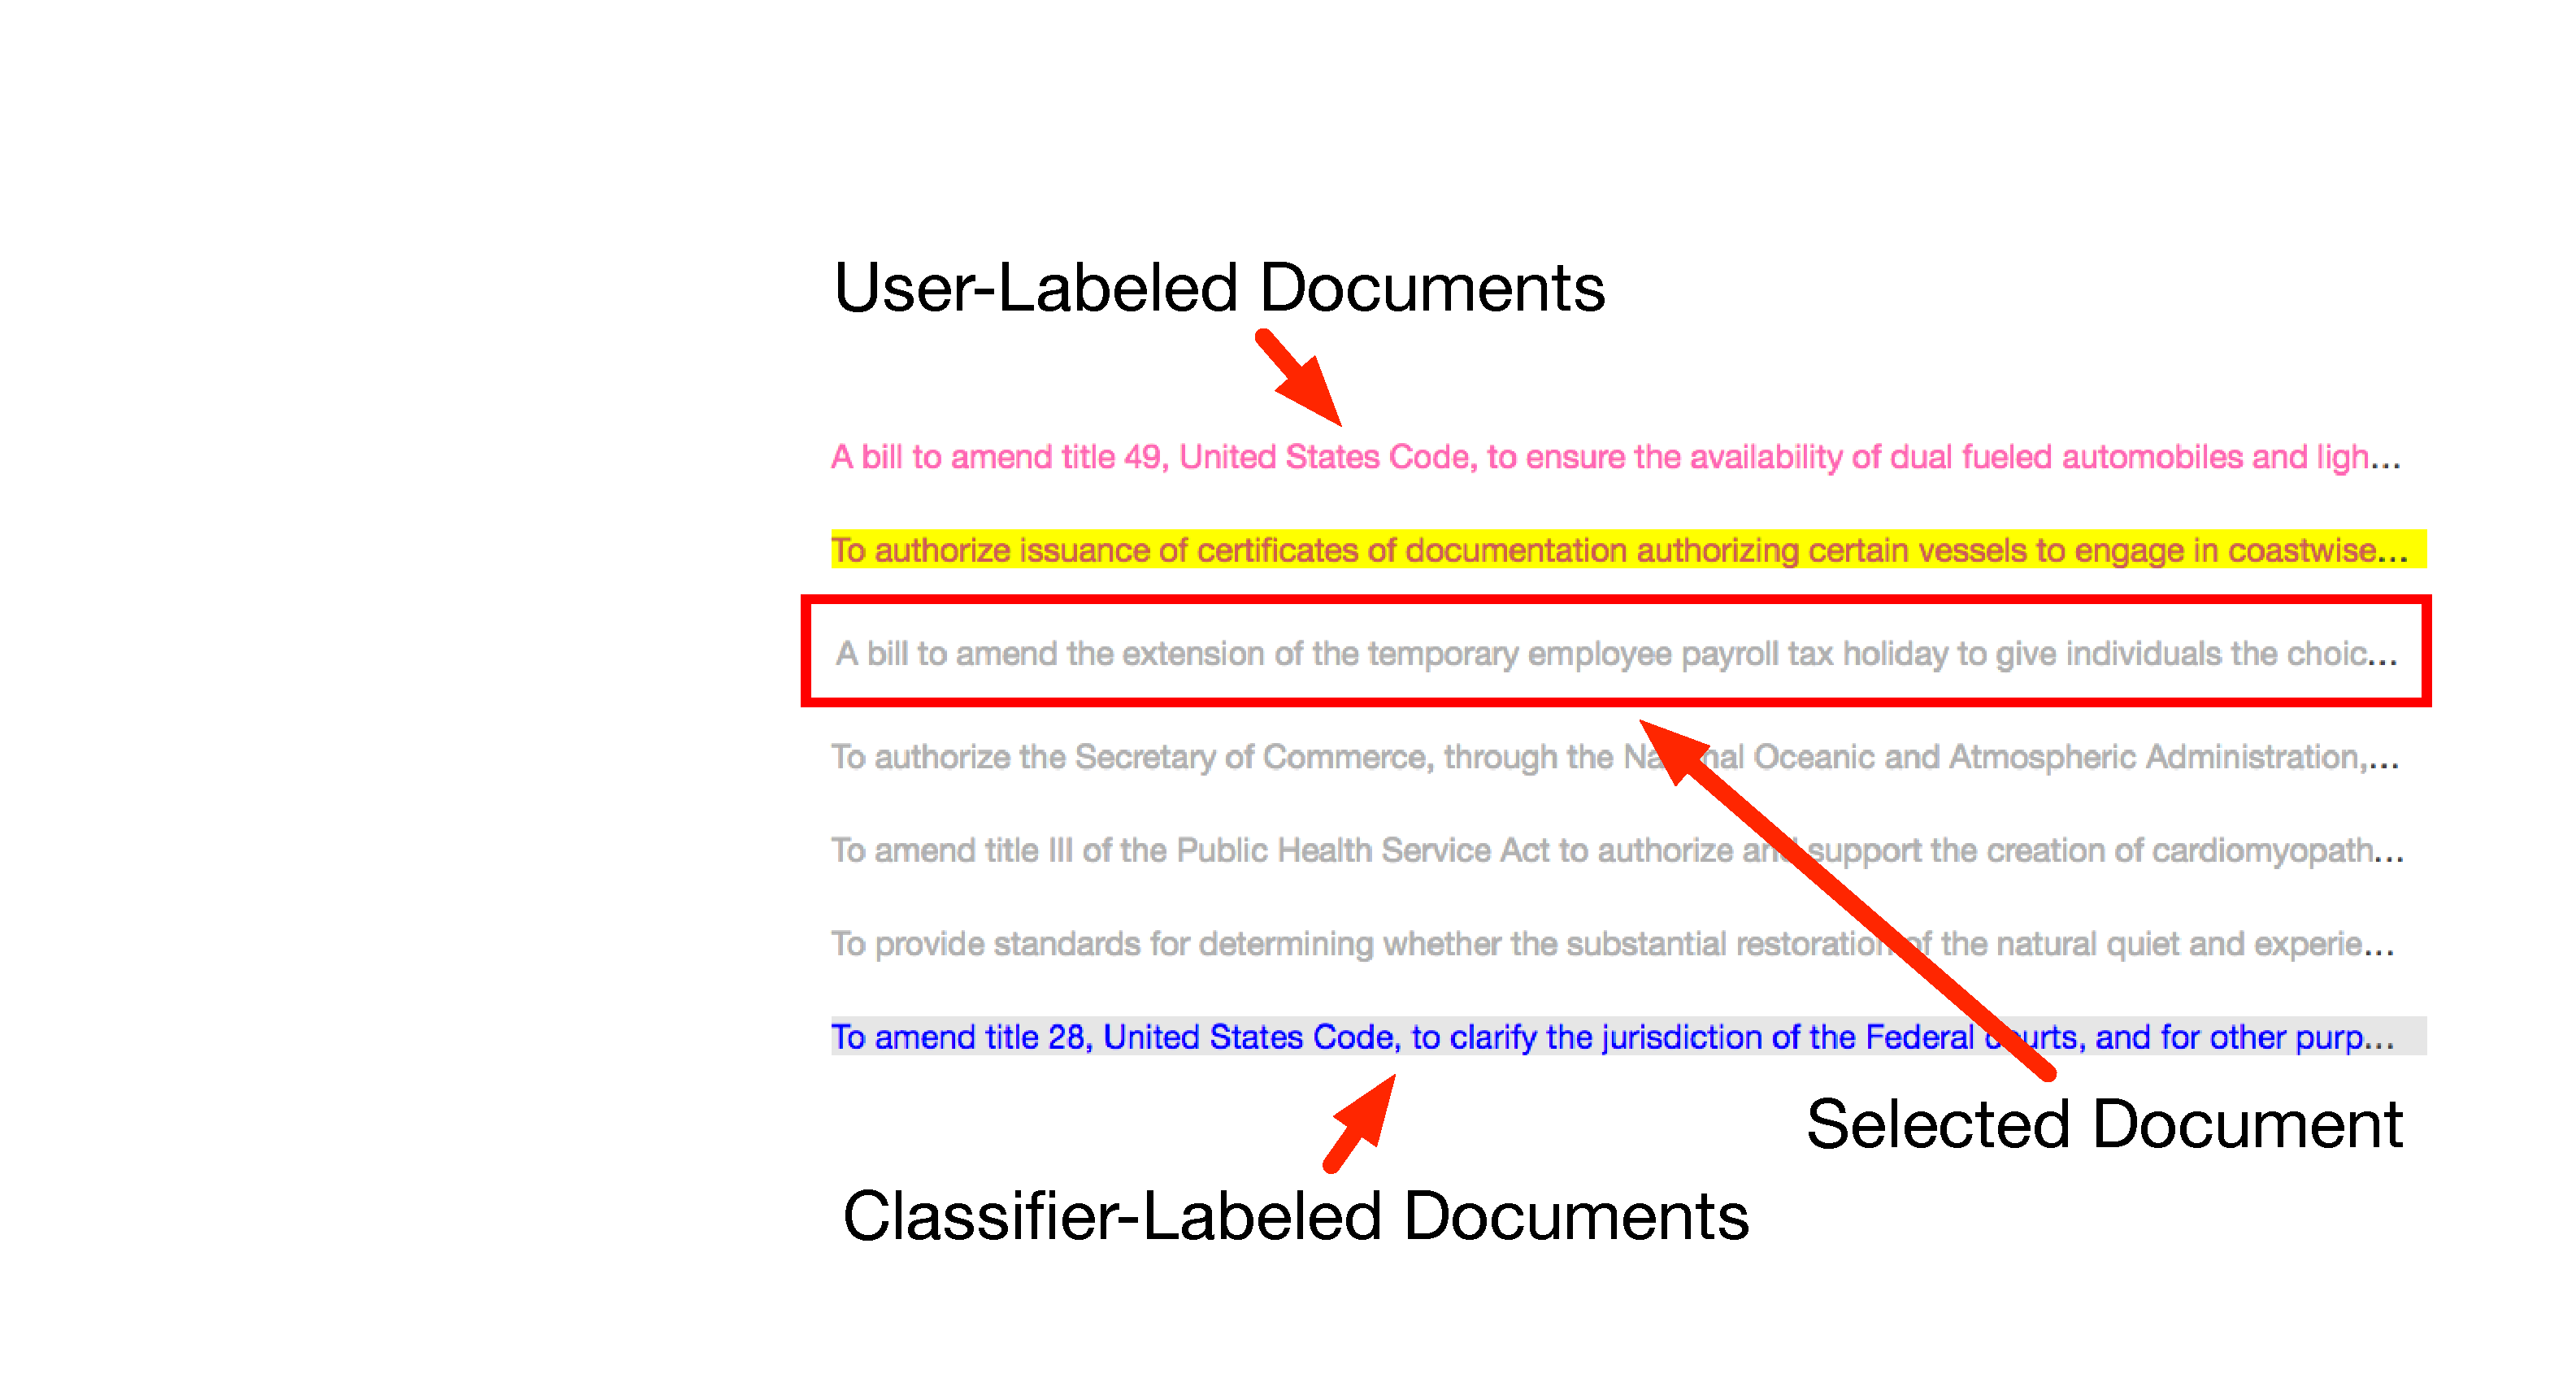
\includegraphics[width=\linewidth]{2016_acl_doclabel/figures/ui_doc_highlight}
  \end{center}
  \caption{After the user has labeled some documents, the system can
    automatically label other documents and select which documents
    would be most helpful to annotate next.  In the random selection
    setting, random documents are selected.}
\label{fig:UI-highlight}
\end{figure}

Our goal is to characterize how local and global knowledge can aid
users in annotating a dataset.  This section describes our four
experimental conditions and outlines the user's process for labeling documents.

\subsection{Study Design}
\label{sub:exp_conditions}





The study uses a $2\times2$ between-subjects design, with factors of
document collection \emph{overview} (two levels: topic model or list)
and document \emph{selection} (two levels: active or random). The four
conditions, with the \abr{ta}
condition representing \name{}, are:
\begin{enumerate*}
  \item Topic model and active selection (\abr{ta})
  \item Topic model and random selection (\abr{tr})
  \item List and active selection (\abr{la})
  \item List and random selection (\abr{lr})
\end{enumerate*}

\subsection{Document Collection Overview}\label{sub:UI}



The topic and list overviews offer different overall structure but the
same basic elements for users to create, modify, and apply labels
(Section~\ref{sub:interaction}). The topic overview
(Figure~\ref{fig:UI-overview}a) builds on \newcite{ITM}: for each
topic, the top twenty words are shown alongside twenty document
titles. Topic words ($w$) are sized based on their probability
$\phi_{k,w}$ in the topic $k$ and the documents with the highest
probability of that topic ($\theta_{d,k}$) are shown.  The list
overview, in contrast, presents documents as a simple, randomly
ordered list of titles (Figure~\ref{fig:UI-overview}b). We
display the same number of documents ($20K$, where $K$ is the total
number of topics) in both the topic model and list overviews, but the
list overview obviously provides no topic information.

\subsection{Document Selection}\label{sub:AL}










To provide consistency across the four conditions, they all use a
document preference function $U$ to direct the user's attention to a document to label.  For the random selection
conditions, \abr{tr} and \abr{lr}, document selection is random, within a topic or globally.
We expect this to be less useful than active
learning. The document preference functions are:

\noindent
\textbf{\abr{la}}: \abr{la} uses traditional uncertainty sampling:
\begin{equation}\label{eq:AL_UA}
	U_{d}^{\mbox{\abr{la}}} = \h{C}{Y_d},
\end{equation}
 where
$\h{C}{y_d} = -\sum_{i} P(y_i|d)log P(y_i|d)$ is the classifier entropy. Entropy measures how confused (uncertain) classifier $C$ is about its prediction of a document $d$'s label $y$. Intuitively, it prefers documents that most of the labels are likely to be predicted to documents that only one of the labels is highly likely to be chosen.
\noindent
\textbf{\abr{lr}}: \abr{lr}'s approach is the same as \abr{la}'s
except we replace $\h{C}{y_d}$ with a uniform random number:
\begin{equation}\label{eq:AL_UR}
	U_{d}^{\mbox{\abr{lr}}} \sim \mbox{unif}(0,1).
\end{equation}
 In contrast to \abr{la}, which suggests the most uncertain document, \abr{lr} suggests a random document.

\noindent
\textbf{\abr{ta}}: \newcite{Dasgupta-08} argue that clustering should inform
active learning criteria, balancing coverage against classifier accuracy.  We
adapt their method to flat topic models---in contrast to their hierarchical
cluster trees---by creating a composite measure of document uncertainty within a
topic:
\begin{equation}
	U_{d}^{\mbox{\abr{ta}}} = \h{C}{y_d} \theta_{d,k},
\label{eq:AL_TA}
\end{equation}
where $k$ is the prominent topic for document $d$. $U_d^{\mbox{\abr{ta}}}$ prefers
documents that are \emph{representative} of a topic
(i.e., have a high value of
$\theta_{d,k}$ for that topic)
and are informative for the classifier.

\noindent
\textbf{\abr{tr}}: \abr{tr}'s approach is the same as \abr{ta}'s
except we replace $\h{C}{Y_d}$ with a uniformly random number:
\begin{equation}\label{eq:AL_TR}
	U_{d}^{\mbox{\abr{tr}}} = \mbox{unif}(0,1) \theta_{d,k}.
\end{equation}
Similar to \abr{ta}, this prefers
documents that are representative of a topic, but not any particular such document. Incorporating the random component encourages for covering different documents in diverse topics.










   In \abr{la} and \abr{lr}, the preference function directly
chooses a document and directs the user to it. On the other hand, $U^{\abr{TA}}_d$
and $U^{\abr{TR}}_d$ are topic dependent: To avoid the negative and misleading effect of topics, users' attention should be drawn to documents that are representative of a specific topic. Therefore, the factor $\theta_{d,k}$ appears in
both. Thus, they require that a topic be chosen first and then the document
with maximum preference, $U$, within that topic can be chosen. In \abr{tr}, the
topic is chosen randomly. In \abr{ta}, the topic is chosen by
\begin{equation}\label{eq:topic_perference}
    k^{*}=\arg\max_k(\mbox{median}_d(\h{C}{y_d} \theta_{d,k}).
\end{equation}
That is the topic with the maximum median $U$. Median encodes how ``confusing'' a topic is.\footnote{Outliers skew other measures (e.g., max or mean).} Intuitively, $k^{*}$ is the topics that the classifier is confused about its documents' labels.

\subsection{User Labeling Process}\label{sub:interaction}





The user's labeling process is the same in all four conditions. The
\emph{overview} (topic or list) allows users to examine individual
documents (Figure~\ref{fig:UI-overview}). Clicking on a document opens a dialog box
(Figure~\ref{fig:UI-label}) with the text of the document and three
options:
\begin{enumerate*}
  \item Create and assign a new label to the document.
  \item Choose an existing label for the document.
  \item Skip the document.
\end{enumerate*}








Once the user has labeled two documents with different labels, the displayed
documents are replaced based on the preference function (Section~\ref{sub:AL}),
every time the user labels (or updates labels for) a document. In \abr{ta} and
\abr{tr}, each topic's documents are replaced with the top twenty most uncertain
documents. In \abr{la} and \abr{lr}, all documents are updated with the top
$20K$ uncertain documents.\footnote{In all conditions, the number of displayed unlabeled documents is adjusted based on the number of manually labeled documents. i.e. if the user has labeled $n$ documents in topic $k$, $n$ manually labeled documents followed by top $20-n$ uncertain documents will be shown in topic $k$.}

The system also suggests one document to
consider by auto-scrolling to it and drawing a red box around its title
(Figure~\ref{fig:UI-highlight}). The user may ignore that document and click on any other
document. After the user labels ten documents, the classifier runs and assigns
labels to other documents.\footnote{To reduce user confusion, for each existing
  label, only the top 100 documents get a label assigned in the \abr{ui}.} For
classifier-labeled documents, the user can either approve the label or assign a
different label. The process continues until the user is satisfied or a time
runs out (forty minutes in our user study, Section~\ref{sec:user_exp_results}).
We use time to control for the varying difficulty of assigning documents: active
learning will select more difficult documents to annotate, but they may be more
useful; time is a more fair basis of comparison in real-world tasks.

\section{Data and Evaluation Metrics}
\label{sec:data_metrics} 
In this section, we describe our data, the machine learning techniques
to learn classifiers from examples, and the evaluation metrics to know
whether the final labeling of the complete documents collection was
successful.

\subsection{Datasets}
\label{sub:data}

\paragraph {Data}

Our experiments require corpora to compare user labels with gold
standard labels. We experiment with two corpora:
20Newsgroups~\cite{20news} and \abr{us} congressional
bills from GovTrack.\footnote{\url{https://www.govtrack.us/}}
















For \abr{us} congressional bills, GovTrack provides bill information
such as the title and text, while the Congressional Bills
Project~\cite{adler2006congressional} provides labels and sub-labels
for the bills. Examples of labels are \underline{agriculture} and
\underline{health}, while sub-labels include \underline{agricultural
  trade} and \underline{comprehensive health care reform}.  The
twenty top-level labels have been developed by consensus over many
years by a team of top political scientists to create a reliable,
robust dataset.  We use the 112\textsuperscript{th} Congress; after
filtering,\footnote{We remove bills that have less than fifty words, no
  assigned gold label, duplicate titles, or have the gold label
  \abr{government operations} or \abr{social welfare}, which are
  broad and difficult for users to label.} this dataset has $5558$
documents.  We use this dataset in both the synthetic experiments
(Section~\ref{sec:synthetic_exp}) and the user study
(Section~\ref{sec:user_exp_results}).


 

The 20 Newsgroups corpus has $19,997$ documents grouped in twenty news
groups that are further grouped into six more general topics. Examples
are \underline{talk.politics.guns} and \underline{sci.electronics},
which belong to the general topics of \underline{politics} and
\underline{science}.  We use this dataset in synthetic experiments
(Section~\ref{sec:synthetic_exp}).

\subsection{Machine Learning Techniques}

\paragraph{Topic Modeling}

To choose the number of topics ($K$), we calculate average topic
coherence~\cite{lau-tealeaves-14} on \abr{us} Congressional Bills, between ten and
forty topics and choose $K=19$, as it has the maximum coherence
score.  For consistency, we use the same number of topics ($K=19$) for 20 Newsgroups corpus. After filtering words based on \abr{tf-idf}, we use
Mallet~\cite{mallet} with default options to learn topics. 



\paragraph{Features and Classification}





A logistic regression
predicts labels for documents and provides the classification uncertainty for
active learning.  To make classification and active learning updates efficient,
we use incremental learning~\cite[LingPipe]{lingpipe}. We update classification parameters
using stochastic gradient descent, restarting with the previously learned
parameters as new labeled documents become available.\footnote{Exceptions are
  when a new label is added, a document's label is deleted, or a label is
  deleted. In those cases, we train the classifier from scratch. Also, for final
  results in Section~\ref{sec:user_exp_results}, we train a classifier from
  scratch.}  We use cross validation on prominent topic as labels to set the parameters for
learning the classifier.\footnote{We use \texttt{blockSize} = $1/\#\textrm{examples}$, \texttt{minEpochs} = 100, \texttt{learningRate} = 0.1, \texttt{minImprovement} = 0.01, \texttt{maxEpochs} = 1000, and \texttt{rollingAverageSize} = 5. The regression is unregularized.}

The features for classification include topic probabilities, unigrams,
and the fraction of labeled documents in each document's prominent
topic. The intuition behind adding this last feature is to allow
active learning to suggest documents in a diverse range of topics if
it finds this feature a useful indicator of
uncertainty.\footnote{However, final classifier's coefficients suggested that this feature did not have a large
  effect.}










 
 

\subsection{Evaluation Metrics}
\label{sub:eval}


 
    Our goal is to create a system that allows users
to quickly induce a high-quality label set.  We compare the
user-created label sets against the data's gold label sets.  Comparing
different clusterings is a difficult task, so we use three clustering
evaluation metrics: purity~\cite{purity}, rand
index~\cite[\abr{ri}]{rand1971objective}, and normalized mutual
information~\cite[\abr{nmi}]{strehl2003cluster}.\footnote{We avoided using adjusted rand index~\cite{hubert1985comparing}, because it can yield negative values, which is not consistent with purity and \abr{nmi}. We also computed
  variation of information~\cite{meilua2003comparing} and normalized
  information distance~\cite{vitanyi2009normalized} and observed consistent trends. We omit these results for the sake of space.}

\paragraph{Purity}

Purity measures how ``pure'' user clusters are compared to gold
clusters. Given each user cluster, it measures what fraction of the documents in a user
cluster belong to the most frequent gold label in that cluster:
\begin{equation}
\label{eq:purity}
\mbox{purity}(\mathbf{U},\mathbf{G}) = \frac{1}{N}\sum\limits_{l} \max\limits_{j}|U_l \cap G_j|,
\end{equation}
where $L$ is the number of labels user creates, $\mathbf{U} = \{U_1,
U_2, \dots,U_L\}$ is the user clustering of documents, $\mathbf{G} =
\{G_1, G_2, \dots, G_J\}$ is gold clustering of documents, and $N$ is
the total number of documents. The user $U_l$ and gold $G_j$ labels
are interpreted as sets containing all documents assigned to that label.

\paragraph{Rand index (\abr{ri})}

\abr{ri} is a \emph{pair counting based} measure, where cluster
evaluation is considered as a series of decisions. If two documents
have the same gold label and the same/different user label (\abr{tp}/\abr{fn}) and if
they do not have the same gold label and are not/are assigned the same user
label (\abr{tn}/\abr{fp}) the decision is right/wrong. \abr{ri} measures the
percentage of decisions that are right:
\begin{equation}
\label{eq:ri}
\mbox{RI} = \frac{TP+TN}{TP+FP+TN+FN}.
\end{equation}

\paragraph{Normalized mutual information (NMI)}
\abr{nmi} is an \emph{information theoretic based} measure that
measures the amount of information one gets about the gold clusters by
knowing what the user clusters are:
\begin{equation}
\label{eq:nmi}
	\mbox{NMI}(\mathbf{U},\mathbf{G})= \frac{2\mathbb{I}(\mathbf{U},\mathbf{G})}{\mathbb{H}_{\mathbf{U}}+\mathbb{H}_{\mathbf{G}}},
\end{equation}
where $\mathbf{U}$ and $\mathbf{G}$ are user and gold clusters,
$\mathbb{H}$ is the entropy and $\mathbb{I}$ is mutual
information~\cite{bouma-09}.


While purity, \abr{ri}, and \abr{nmi} are all normalized within $[0,1]$
(higher is better), they measure different things.  Purity measures
the intersection between two clusterings, it is sensitive to the
number of clusters, and it is not symmetric. 
  
  On the other hand, \abr{ri} and
\abr{nmi} are less sensitive to the number of clusters and are
symmetric. \abr{ri} measures pairwise agreement in contrast to purity
that directly measures intersection. Moreover, \abr{nmi} measures
shared information between two clusterings.

None of these metrics are perfect: purity can be exploited by putting
each document in its own label, \abr{ri} does not distinguish
separating similar documents with distinct labels from giving dissimilar documents
the same label, and \abr{nmi}'s ability to compare different numbers of clusters
means that it sometimes gives high scores for clusterings by
chance. Given the diverse nature of these metrics, if a labeling does
well in all three of them, we can be relatively confident that it is not
a degenerate solution that games the system.










\section{Synthetic Experiments}
\label{sec:synthetic_exp}
 
\begin{figure}[t!]
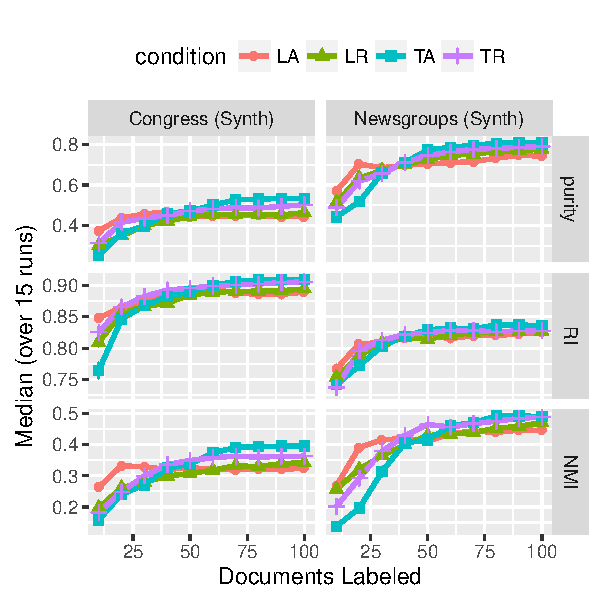
\includegraphics[width=\linewidth]{2016_acl_doclabel/auto_fig/synthetic}
\caption{Synthetic results on \abr{us} Congressional
  Bills and 20 Newsgroups data sets.  Topic models help guide annotation
  attention to diverse segments of the data.}
\label{fig:syn_results}
\end{figure}
Before running a user study, we test our hypothesis that topic
model overviews and active learning selection improve final cluster quality compared to standard baselines: list overview and random
selection. We simulate the four conditions on Congressional
Bills and 20 Newsgroups.

Since we believe annotators create more specific labels compared to the gold
labels, we use sub-labels as simulated user labels and labels as gold labels (we
give examples of labels and sub-labels in Section~\ref{sub:data}). We start with
two randomly selected documents that have different sub-labels, assign the
corresponding sub-labels, then add more labels based on each condition's
preference function (Section~\ref{sub:AL}).  We follow the condition's
preference function and incrementally add labels until 100 documents have been
labeled (100 documents are representative of what a human can label in about an
hour).  Given these labels, we compute purity, \abr{ri}, and \abr{nmi} over
time. This procedure is repeated fifteen times (to account for the randomness of
initial document selections and the preference functions with
randomness).\footnote{Synthetic experiment data available at
\let\hyper@linkurl\saved@hyper@linkurl
  \url{http://github.com/Pinafore/publications/tree/master/2016_acl_doclabel/data/synthetic_exp}
  \NoHyper
  }

Synthetic results validate our hypothesis that topic overview and active learning selection can help label a corpus more efficiently
(Figure~\ref{fig:syn_results}).  \abr{la} shows early gains, but
tends to falter eventually compared to both topic overview and topic overview  combined with active learning selection (\abr{tr} and \abr{ta}).


However, these experiments do not validate \name{}.  Not all documents
require the same time or effort to label, and active learning focuses
on the hardest examples, which may confuse users.  Thus, we need to
evaluate how effectively actual users annotate a collection's
documents.


\section{User Study}
\label{sec:user_exp_results}\begin{figure}[t!]
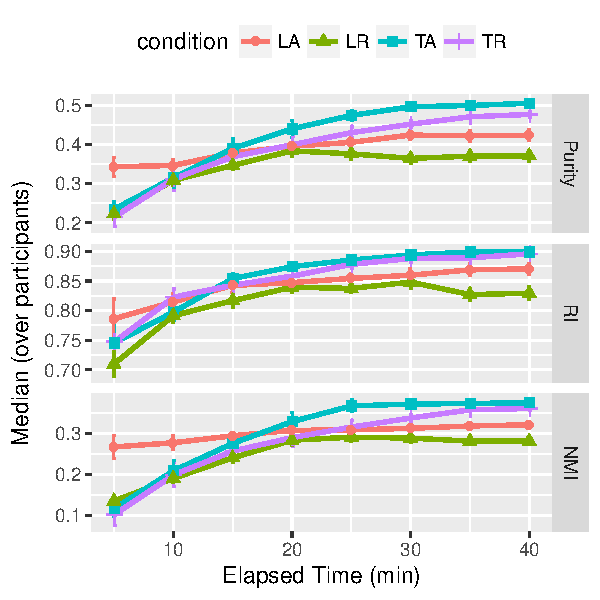
\includegraphics[width=\linewidth]{2016_acl_doclabel/auto_fig/user_exp_plot}
\caption{User study results on \abr{us} Congressional Bills dataset. Active learning selection helps initially, but the combination of active learning selection and topic model overview has highest quality labels by the end of the task.}
\label{fig:results}
\end{figure}

Following the synthetic experiments, we conduct a user study with
forty participants to evaluate \name{} (\abr{ta} condition) against
three alternatives that lack topic overview (\abr{la}), active
learning selection (\abr{tr}), or both (\abr{lr}) (Sections~\ref{sub:procedures} and~\ref{sub:cluster_results}). Then, we conduct a crowdsourced study to compare the overall effectiveness of the label set generated by the participants in the four conditions (Section~\ref{sub:label_results}).

\subsection{Method}
\label{sub:procedures}

We use the freelance marketplace Upwork to recruit online
participants.\footnote{
\let\hyper@linkurl\saved@hyper@linkurl
\url{http://Upwork.com}\NoHyper} We require participants to have
more than $90\%$ job success on Upwork, English fluency, and \abr{us}
residency. Participants are randomly assigned to one of the four conditions and
we recruited ten participants per condition.

Participants completed a demographic questionnaire, viewed a video of task
instructions, and then interacted with the system and labeled documents until
satisfied with the labels or forty minutes had elapsed.\footnote{Forty minutes
  of activity, excluding system time to classify and update
  documents. Participants nearly exhausted the time: $39.3$
 average minutes in \abr{ta}, $38.8$ in \abr{tr}, $40.0$ in \abr{la}, and $35.9$ in
  \abr{lr}.} The session ended with a survey, where participants rated mental,
physical, and temporal demand, and performance, effort, and frustration on
20-point scales, using questions adapted from the \abr{nasa} Task Load
Index~\cite[\abr{tlx}]{hart1988development}. The survey also included 7-point
scales for ease of coming up with labels, usefulness and satisfaction with the
system, and---for \abr{tr} and \abr{ta}---topic information helpfulness. Each
participant was paid fifteen dollars.\footnote{User study data available at
\let\hyper@linkurl\saved@hyper@linkurl
  \url{http://github.com/Pinafore/publications/tree/master/2016_acl_doclabel/data/user_exp}
  \NoHyper
  }

For statistical analysis, we primarily use $2\times2$ (\emph{overview} $\times$
\emph{selection}) \abr{anova}s with Aligned Rank
Transform~\cite[\abr{art}]{wobbrock2011aligned}, which is a non-parametric
alternative to a standard \abr{anova} that is appropriate when data are not
expected to meet the normality assumption of \abr{anova}.
















\subsection{Document Cluster Evaluation}
\label{sub:cluster_results}





We analyze the data by dividing the forty-minute labeling task into
five minute intervals. If a participant stopped before the time
limit, we consider their final dataset to stay the same for any
remaining intervals. Figure~\ref{fig:results} shows the
measures across study conditions, with similar trends for all three
measures.

\paragraph{Topic model overview and active learning both significantly improve final dataset measures.}

The topic overview and active selection conditions significantly
outperform the list overview and random selection, respectively, on
the final label quality metrics. Table~\ref{tab:stats} shows the
results of separate $2\times2$ \abr{anova}s with \abr{art} with each
of final purity, \abr{ri}, and \abr{nmi} scores. There are significant main
effects of \emph{overview} and \emph{selection} on all three metrics;
no interaction effects were significant.






\begin{table}[t!]
\small
\resizebox{\columnwidth}{!}{
\begin{tabular}{*5c}
    \hline
    & \multicolumn{2}{c}{$F$} & \multicolumn{2}{c}{$p$} \\
    & Overview & Selection & Overview & Selection
    \tabularnewline \hline \hline
	final purity & 81.03& 7.18 & $< .001$ & $.011$
    \tabularnewline
    \hline
	final \abr{ri} & 39.89 & 6.28 &  $<.001$ & $.017$
\tabularnewline
\hline
	final \abr{nmi} &70.92 &9.87 & $<.001$ & $.003$
 \tabularnewline
\hline
	\multicolumn{5}{c}{df(1,36) for all reported results}
\end{tabular}
}
\caption{Results from $2\times2$ \abr{anova} with \abr{art} analyses on the
final purity, \abr{ri}, and \abr{nmi} metrics. Only main effects for
the factors of \emph{overview} and \emph{selection} are shown; no interaction
effects were statistically significant.  Topics and active learning
both had significant effects on quality scores.}
\label{tab:stats}
\end{table}

\paragraph{\abr{tr} outperforms \abr{la}.}

Topic models by themselves outperform traditional active learning
strategies (Figure~\ref{fig:results}).  \abr{la} performed
better than \abr{lr}; while active learning was useful, it was not as
useful as the topic model overview (\abr{tr} and \abr{ta}).





\paragraph{\abr{la} provides an initial benefit.}

Average purity, \abr{nmi} and \abr{ri} were highest with \abr{la} for
the earliest labeling time intervals.  Thus, when time is very
limited, using traditional active learning (\abr{la}) is preferable to
topic overviews; users need time to explore the topics and a subset of
documents within them. Table~\ref{tab:early_results} shows the metrics
after ten minutes. Separate $2\times2$ \abr{anova}s with \abr{art} on
the means of purity, \abr{nmi} and \abr{ri} revealed a significant
interaction effect between \emph{overview} and \emph{selection} on
mean \abr{nmi} ($F(1,36)= 5.58$, $p$ = $.024$), confirming the early
performance trends seen in Figure~\ref{fig:results} at least for
\abr{nmi}. No other main or interaction effects were significant,
likely due to low statistical power.

\begin{table}[t!]
\small
\resizebox{\columnwidth}{!}{
\begin{tabular}{*4c}
    \hline
    & \multicolumn{3}{c}{$M \,\,\pm\,\, SD \,[median]$} \\
    &purity & \abr{ri} & \abr{nmi}
    \tabularnewline \hline \hline
	\abr{ta} & $0.31 \,\pm\, 0.08 \,[0.32]$& $0.80 \,\pm\, 0.05 \,[0.80]$ & $0.19 \,\pm\, 0.08 \,[0.21]$
    \tabularnewline
    \hline
	\abr{tr} & $0.32 \,\pm\, 0.09 \,[0.31]$& $0.82 \,\pm\, 0.04 \,[0.82]$ &  $0.21 \,\pm\, 0.09 \,[0.20]$
\tabularnewline
\hline
	\abr{la} &$0.35 \,\pm\, 0.05 \,[0.35]$ & $0.82 \,\pm\, 0.04 \,[0.81]$ & $0.27 \,\pm\, 0.05 \,[0.28]$
 \tabularnewline \hline
	\abr{lr} &$0.31 \,\pm\, 0.04 \,[0.31]$ &$0.79 \,\pm\, 0.04 \,[0.79]$ & $0.19 \,\pm\, 0.03 \,[0.19]$
	 \tabularnewline \hline
\end{tabular}
}
\caption{Mean, standard deviation, and median purity, \abr{ri}, and \abr{nmi}
  after ten minutes. \abr{nmi} in particular shows the benefit of \abr{la} over other conditions at early time intervals.}
\label{tab:early_results}
\end{table}



\begin{table*}[t!]
\resizebox{\textwidth}{!}{
\begin{tabular}{*7c}
    \hline
        & \multicolumn{6}{c}{$M \,\,\pm\,\, SD \,[median]$} \\
    Condition & Mental Demand & Physical Demand & Temporal Demand & Performance & Effort & Frustration
    \tabularnewline \hline \hline
	\abr{ta} &$9.8 \,\,\pm\,\, 5.6 \,[10]$&$2.9 \,\,\pm\,\, 3.4 \,[2]$&$9 \,\,\pm\,\, 7.8 \,[7$]&$5.5 \,\,\pm\,\, 5.8 \,[1.5]$&$9.4 \,\,\pm\,\, 6.3 \,[10]$&$4.5 \,\,\pm\,\, 5.5 \,[1.5]$

    \tabularnewline
    \hline
	\abr{tr} &$10.6 \,\,\pm\,\, 4.5 \,[11]$&$2.4 \,\,\pm\,\, 2.8 \,[1]$&$7.4 \,\,\pm\,\, 4.1 \,[9]$&$8.8 \,\,\pm\,\, 6.1 \,[7.5]$&$9.8 \,\,\pm\,\, 3.7 \,[10]$&$3.9 \,\,\pm\,\, 3.0 \,[3.5]$

\tabularnewline
\hline
	\abr{la} &$9.1 \,\,\pm\,\, 5.5 \,[10]$&$1.7 \,\,\pm\,\, 1.3 \,[1]$&$10.2 \,\,\pm\,\, 4.8 \,[11]$&$8.6 \,\,\pm\,\, 5.3 \,[10]$&$10.7 \,\,\pm\,\, 6.2 \,[12.5]$&$6.7 \,\,\pm\,\, 5.1 \,[5.5]$

 \tabularnewline
\hline
	\abr{lr} &$9.8 \,\,\pm\,\, 6.1 \,[10]$&$3.3 \,\,\pm\,\, 2.9 \,[2]$&$9.3 \,\,\pm\,\, 5.7 \,[10]$&$9.4 \,\,\pm\,\, 5.6 \,[10]$&$9.4 \,\,\pm\,\, 6.2 \,[10]$&	$7.9 \,\,\pm\,\, 5.4 \,[8]$
 \tabularnewline
\hline
\end{tabular}
}
\caption{
Mean, standard deviation, and median results from \abr{nasa-tlx}
 post-survey. All questions are scaled 1 (low)--20 (high), except performance, which is scaled 1 (good)--20 (poor). Users found topic model overview conditions, \abr{tr} and \abr{ta}, to be significantly less frustrating than the list overview conditions.}
\label{tab:NASA_res}
\end{table*}

\paragraph{Subjective ratings.}

Table~\ref{tab:NASA_res} shows the average scores given for the six
\abr{nasa-tlx} questions in different conditions. Separate $2\times2$
\abr{anova} with \abr{art} for each of the measures revealed only one
significant result: participants who used the topic model overview find the
task to be significantly less frustrating (\mbox{$M=4.2$} and \mbox{$median=2$})
than those who used the list overview (\mbox{$M=7.3$} and \mbox{$median=6.5$})
on a scale from 1 (low frustration) to 20 (high frustration)
(\mbox{$F(1,36)=4.43$}, \mbox{$p=.042$}), confirming that the topic overview
helps users organize their thoughts and experience less stress during labeling.

Participants in the \abr{ta} and \abr{tr} conditions rate topic
information to be useful in completing the task (\mbox{$M=5.0$} and
\mbox{$median=5$}) on a scale from 1 (not useful at all) to 7 (very
useful).  Overall, users were positive about their experience with the
system. Participants in all conditions rated overall satisfaction
with the interface positively (\mbox{$M=5.8$ and $median=6$}) on a
scale from 1 (not satisfied at all) to 7 (very satisfied).
\paragraph{Discussion}

One can argue that using topic overviews for labeling could have a negative effect:
users may ignore the document content and focus on topics for labeling. We tried
to avoid this issue by making it clear in the instructions that they need to
focus on document content and use topics as a guidance. On average, the participants in
\abr{tr} created 1.96 labels per topic and the participants in \abr{ta} created
2.26 labels per topic. This suggests that participants are going beyond what
they see in topics for labeling, at least in the \abr{ta} condition.









\subsection{Label Evaluation Results}
\label{sub:label_results}

Section~\ref{sub:cluster_results} compares clusters of documents in different
conditions against the gold clustering but ignores what the labels
actually are. To assess how the final induced label sets compare in
different conditions, we use crowdsourcing to assess the quality of
documents' labels.  

For completeness, we also compare labels against a fully automatic
labeling method~\cite{aletras2014labelling} that does not require
human intervention.  We assign \emph{automatic} labels to documents
based on their most prominent topic.

We ask users on a crowdsourcing platform to \emph{vote} for the ``best'' and
``worst'' label that describes the content of a \abr{us} congressional
bill (we use Crowdflower and require contributors to be in the \abr{us}).

Five users label each document and we use the aggregated results generated by
Crowdflower. The user gets \$0.20 for each task. 

We randomly choose $200$ documents from our dataset (Section
\ref{sub:data}). For each chosen document, we randomly choose a participant from
all four conditions (\abr{ta}, \abr{tr}, \abr{la}, \abr{lr}). The labels
assigned in different conditions and the automatic label of the document's prominent
topic construct the candidate labels for the document.\footnote{Some
  participants had typos in the labels. We corrected all the typos using
  pyEnchant (\let\hyper@linkurl\saved@hyper@linkurl \url{http://pythonhosted.org/pyenchant/} \NoHyper) spellchecker. If the
  corrected label was still wrong, we corrected it manually.} Identical labels are
merged into one label to avoid showing duplicate labels to users. If a merged
label gets a ``best'' or ``worst'' vote, we split that vote across all the
identical instances.\footnote{
Evaluation data available at \let\hyper@linkurl\saved@hyper@linkurl\url{http://github.com/Pinafore/publications/tree/master/2016_acl_doclabel/data/label_eval} \NoHyper
}
Figure~\ref{fig:eval_votes} shows the average number of ``best'' and ``worst''
votes for each condition and the automatic method.
\name{} (\abr{ta}) receives the most ``best'' votes and the fewest
``worst'' votes. \abr{lr} receive the most worst votes. The automatic labels, interestingly, appear to do at least as well as the list view labels, with a similar number of best votes and fewer worst votes.  This indicates that automatic labels have reasonable quality compared to at least some manually generated labels. However, when users are provided with topic model overview, with or
without active learning selection, they can generate label sets that
 improve upon automatic labels and labels assigned without the topic
model overview.













\begin{figure}[t!]
 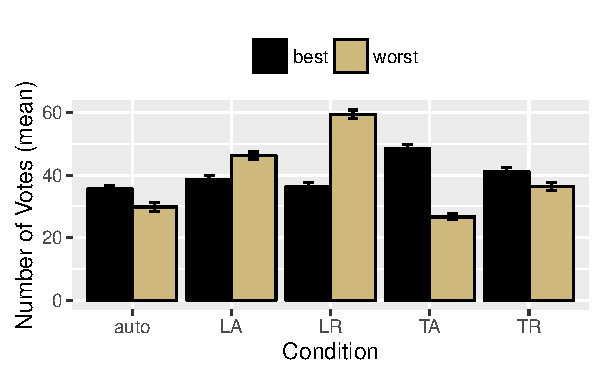
\includegraphics[width=0.5\textwidth]{2016_acl_doclabel/auto_fig/eval_votes}
 \caption{Best and worst votes for document labels. Error
   bars are standard error from bootstrap sample. \name{}
   (\abr{ta}) gets the most best votes and the fewest worst votes.}
\label{fig:eval_votes}
\end{figure}

\section{Related Work}
\label{sec:related_work}




















Text classification---a ubiquitous machine learning tool for
classifying text~\cite{zhang-10}---requires feature
extraction~\cite{lewis1992feature}. These are both well-trodden areas
of \abr{nlp} research.  The difficulty is often creating the training
data~\cite{hwa2004sample,osborne2004ensemble}; coding theory is an
entire subfield of social science devoted to creating, formulating, and applying labels to text data~\cite{saldana-12,musialek-16}.
Crowdsourcing~\cite{snow-08} and active
learning~\cite{settles2012active}, can decrease the cost of annotation
but only \emph{after} a label set exists.

\nocite{iyyer2014political,anand2011believe,nikolova2011collecting}

\name{} quantitatively shows that corpus overviews aid text
understanding, building on traditional interfaces for gaining both
local and global information~\cite{hearst-96}.  More elaborate
interfaces~\cite{eisenstein-12,chaney-12} provide richer information given a fixed topic model.
Alternatively, because topic models are imperfect~\cite{boyd2014care},
refining underlying topic models may also improve users'
understanding of a corpus~\cite{choo-13,hoque-15}.

Summarizing document collections through discovered topics can happen
through raw topics labeled manually by users~\cite{talley-11}, automatically~\cite{lau-11}, or by learning a mapping
from labels to topics~\cite{ramage-09}.  When there is not a direct
correspondence between topics and labels, classifiers learn a
mapping~\cite{blei-07b,zhu-09,Nguyen:Boyd-Graber:Lund:Seppi:Ringger-2015}.
Because we want topics to be consistent between users, we use a
classifier with static topics in \name{}. \name{} combines active
learning with topic models to provide both global and local knowledge
document labeling requires.








\section{Conclusion and Future Work}
\label{sec:conclusion}









We introduce \name{}, an interactive framework that combines active
learning \emph{selection}s with topic model \emph{overview}s to help
users induce a label set and label documents. We show that users can
more effectively and efficiently induce label set and create training
data using \name{} in comparison with other conditions, which lack
either topic \emph{overview} or active \emph{selection}.

We can further improve \name{} (the \abr{ta} condition) to help users gain
better and faster understanding of text corpora.  Our current system limits
users to view only $20K$ documents at a time and allows for one label assignment
per document. Moreover, the topics are static and do not adapt to better reflect
users' labels. Users should have better support for browsing documents and
assigning multiple labels.  Topics can also improve
via \abr{slda}~\cite{blei-07b} or
\abr{llda}~\cite{ramage2009labeled} as users add labels.

Finally, with slight changes to what the system
considers a document, we believe \name{} can be extended to \abr{nlp} applications
other than classification, such as named entity recognition or
semantic role labeling, to reduce the annotation effort.


\clearpage

\section*{Acknowledgments}
We thank the anonymous reviewers, Philip Resnik, and Burr Settles for
their insightful comments. We also thank Nikolaos Aletras for
providing the automatic topic labeling code.  Boyd-Graber and
Poursabzi-Sangdeh's contribution is supported by \abr{nsf} Grant
\abr{ncse}-1422492; Findlater, Seppi, and Boyd-Graber's contribution
is supported by collaborative \abr{nsf} Grant \abr{iis}-1409287
(\abr{umd}) and \abr{iis}-1409739 (\abr{byu}).  Any opinions,
findings, results, or recommendations expressed here are of the
authors and do not necessarily reflect the view of the sponsor.

\bibliographystyle{style/acl2016}
\bibliography{bib/journal-full,bib/jbg,bib/forough}




\end{document}
